\documentclass[10pt,twocolumn,letterpaper]{article}

\usepackage[labelfont=bf]{caption}
\usepackage[table]{xcolor}
\usepackage{graphicx}
\usepackage{multirow}
\usepackage{amsfonts}
\usepackage{amssymb}
\usepackage[tbtags]{amsmath}
\usepackage[a4paper,margin=4cm]{geometry}
\usepackage{lastpage}
\usepackage{fancyhdr}
\usepackage[round]{natbib}
\usepackage{listings}
\usepackage{color}
\usepackage[title]{appendix}
\usepackage{bm}
\usepackage{textcomp}
\usepackage{mathtools}
\usepackage{tabularx}
\usepackage{booktabs}
\usepackage{ragged2e}
\usepackage{float}
\usepackage{enumitem}
\usepackage{tabularx}
\usepackage{tikz}
\usetikzlibrary{fit, shapes.misc, positioning, arrows.meta, calc}

\bibliographystyle{plainnat}
\def\sumin{\sum_{i=1}^{n}}
\def\bhline{\noalign{\hrule height 1pt}}

\DeclarePairedDelimiter\abs{\lvert}{\rvert}

%table
\captionsetup[table]{skip=0pt}
\definecolor{faintgrey}{RGB}{242, 242, 242}
\def\evenrow{\rowcolor{faintgrey}}
\newcolumntype{L}{>{\raggedright\arraybackslash}X}
\newcolumntype{C}{>{\centering\arraybackslash}X}
\newcolumntype{P}{>{\raggedright\arraybackslash}p}

%notations
\def\nodedistance{0.3cm}
\definecolor{fc}{RGB}{251, 227, 214}
\definecolor{fc-relu}{RGB}{246, 198, 173}
\definecolor{lstm}{RGB}{180, 229, 162}
\definecolor{drop-out}{RGB}{217, 217, 217}
\definecolor{input}{RGB}{97, 203, 244}

\tikzstyle{arrow} = [gray, -{Triangle[angle=45:1pt 3]}, line width=1.5pt]
\tikzstyle{thin-arrow} = [gray, -{Straight Barb[angle'=60,scale=2]}, line width=0.8pt]
\tikzstyle{connector} = [gray, -, >=stealth, line width=1.5pt]

\newcommand{\unitw}[2]{w_{#2}^{(#1)}}
\newcommand{\tikzlayernode}[1]{\node[
  draw=none, rounded rectangle, minimum width=0.62cm, minimum height=0.43cm, fill=#1, inner sep=0,
  font=\fontsize{8pt}{8pt}\selectfont
]}
\newcommand{\tikzinputnode}[1]{\node[
  draw=none, circle, minimum height=0.43cm, fill=#1, inner sep=0, font=\fontsize{8pt}{8pt}\selectfont
]}

\newcommand{\nnlayer}[2]{\begin{tikzpicture}[baseline=-0.1cm]
  \tikzlayernode{#1}{#2};
\end{tikzpicture}}

\newcommand{\nninput}[2]{\begin{tikzpicture}[baseline=-0.1cm]
  \tikzinputnode{#1}{#2};
\end{tikzpicture}}

%architectures
\newcommand{\architecturea}[1]{
  \begin{tikzpicture}[node distance=\nodedistance, baseline=#1]
    % nodes
    \tikzinputnode{input} at (0, 0)           (input)   {};
    \tikzlayernode{lstm}  [right = of input]  (1)       {400};
    \tikzinputnode{fc}    [right = of 1]      (output)  {5};

    % arrows
    \draw[connector]  (input) -- (1);
    \draw[arrow]      (1)     -- (output);
  \end{tikzpicture}
}
\newcommand{\architectureb}[1]{
  \begin{tikzpicture}[node distance=\nodedistance, baseline=#1]
    % nodes
    \tikzinputnode{input} at (0, 0)           (input)   {};
    \tikzlayernode{lstm}  [right = of input]  (1)       {200};
    \tikzinputnode{fc}    [right = of 1]      (output)  {5};

    % arrows
    \draw[connector]  (input) -- (1);
    \draw[arrow]      (1)     -- (output);
  \end{tikzpicture}
}
\newcommand{\architecturec}[1]{
  \begin{tikzpicture}[node distance=\nodedistance, baseline=#1]
    % nodes
    \tikzinputnode{input} at (0, 0)           (input)   {};
    \tikzlayernode{lstm}  [right = of input]  (1)       {100};
    \tikzinputnode{fc}    [right = of 1]      (output)  {5};

    % arrows
    \draw[connector]  (input) -- (1);
    \draw[arrow]      (1)     -- (output);
  \end{tikzpicture}
}
\newcommand{\architectured}[1]{
  \begin{tikzpicture}[node distance=\nodedistance, baseline=#1]
    % nodes
    \tikzinputnode{input}     at (0, 0)           (input)   {};
    \tikzlayernode{lstm}      [right = of input]  (1)       {400};
    \tikzlayernode{drop-out}  [right = of 1]      (2)       {0.2};
    \tikzlayernode{lstm}      [right = of 2]      (3)       {200};
    \tikzlayernode{fc-relu}   [right = of 3]      (4)       {64};
    \tikzinputnode{fc}        [right = of 4]      (output)  {5};

    % arrows
    \draw[connector]  (input) -- (1);
    \draw[connector]  (1)     -- (2);
    \draw[connector]  (2)     -- (3);
    \draw[connector]  (3)     -- (4);
    \draw[arrow]      (4)     -- (output);
  \end{tikzpicture}
}
\newcommand{\architecturee}[1]{
  \begin{tikzpicture}[node distance=\nodedistance, baseline=#1]
    % nodes
    \tikzinputnode{input}     at (0, 0)           (input)   {};
    \tikzlayernode{lstm}      [right = of input]  (1)       {200};
    \tikzlayernode{drop-out}  [right = of 1]      (2)       {0.2};
    \tikzlayernode{lstm}      [right = of 2]      (3)       {100};
    \tikzlayernode{fc-relu}   [right = of 3]      (4)       {64};
    \tikzinputnode{fc}        [right = of 4]      (output)  {5};

    % arrows
    \draw[connector]  (input) -- (1);
    \draw[connector]  (1)     -- (2);
    \draw[connector]  (2)     -- (3);
    \draw[connector]  (3)     -- (4);
    \draw[arrow]      (4)     -- (output);
  \end{tikzpicture}
}
\newcommand{\architecturef}[1]{
  \begin{tikzpicture}[node distance=\nodedistance, baseline=#1]
    % nodes
    \tikzinputnode{input}     at (0, 0)           (input)   {};
    \tikzlayernode{lstm}      [right = of input]  (1)       {400};
    \tikzlayernode{drop-out}  [right = of 1]      (2)       {0.2};
    \tikzlayernode{lstm}      [right = of 2]      (3)       {200};
    \tikzinputnode{fc}        [right = of 3]      (output)  {5};

    % arrows
    \draw[connector]  (input) -- (1);
    \draw[connector]  (1)     -- (2);
    \draw[connector]  (2)     -- (3);
    \draw[arrow]      (3)     -- (output);
  \end{tikzpicture}
}
\newcommand{\architectureg}[1]{
  \begin{tikzpicture}[node distance=\nodedistance, baseline=#1]
    % nodes
    \tikzinputnode{input}     at (0, 0)           (input)   {};
    \tikzlayernode{lstm}      [right = of input]  (1)       {200};
    \tikzlayernode{drop-out}  [right = of 1]      (2)       {0.2};
    \tikzlayernode{lstm}      [right = of 2]      (3)       {100};
    \tikzinputnode{fc}        [right = of 3]      (output)  {5};

    % arrows
    \draw[connector]  (input) -- (1);
    \draw[connector]  (1)     -- (2);
    \draw[connector]  (2)     -- (3);
    \draw[arrow]      (3)     -- (output);
  \end{tikzpicture}
}

% Include other packages here, before hyperref.

% If you comment hyperref and then uncomment it, you should delete
% egpaper.aux before re-running latex.  (Or just hit 'q' on the first latex
% run, let it finish, and you should be clear).
\usepackage[breaklinks=true,bookmarks=false]{hyperref}

\def\httilde{\mbox{\tt\raisebox{-.5ex}{\symbol{126}}}}

% Pages are numbered in submission mode, and unnumbered in camera-ready
%\ifcvprfinal\pagestyle{empty}\fi
%\setcounter{page}{4321}
\begin{document}

%%%%%%%%% TITLE
\title{Assessment 3: RNNs for Stock Price Prediction}

\author{Wasin Pipattungsakul \\
The University of Adelaide \\
{\tt\small wasin.pipattungsakul@adelaide.edu.au}
}

\maketitle
%\thispagestyle{empty}

%%%%%%%%% ABSTRACT
\begin{abstract}
  This work investigates the performance of long short-term memory neural network models on Goole Stock Price
  dataset. The models were designed with different number and types of layers to observe the impact of different
  layers. Predictions were made on open, close, high, and low prices for the next 5 days. There were no obvious
  variations in performance between different predicted prices.
\end{abstract}

%%%%%%%%% BODY TEXT
\section{Introduction}

In this work, the performance of neural network (NN) models with long short-term memory (LSTM) layers on Google
Stock Price dataset \citep{data}. Different architectures with several configurations were trained for best
mean squared error (MSE) on a validation set with these target parameters, open, close, high, and low prices.
The predictions were 5 days into the future, so traders can plan their strategies for the whole week if the
results were promising.

%-------------------------------------------------------------------------
\subsection{Google Stock Price}

According to \citet{data}, the Google Stock Price dataset consists of 1,258 records of open, close, high, and
low prices and volume on trading days for a training set. A test set consists of 20 records.

%-------------------------------------------------------------------------
\subsection{LSTM}

LSTM layers can address the vanishing error issue that often happens in normal recurrent neural network (RNN)
from possible repetitive shrinking weights during back propagation in multiple steps \citep{lstm}. LSTM layers
allow constant error flow through its internal architecture. The detail is not presented in this work, but it
can be explored further in the cited article.

%------------------------------------------------------------------------
\section{Methods}

%-------------------------------------------------------------------------
\subsection{Data}

As a part of exploratory data analysis (EDA), simple plots were drawn for Google Stock Price dataset to check
whether the data is sound and there is no anomaly. Otherwise, imputation or transformations would be applied
where needed.

The dataset was then split into multiple configurations based on
\begin{enumerate}
  \item the number of days observed before the prediction and
  \item the number of days in the future to be predicted.
\end{enumerate}
In this work, we predicted only 5 days into the future. The split configurations ensure that there were no data
leakage from the validation set in the train set and from the test set in the validation set. The splits are
presented in table
\ref{tab:split-configurations}.
\begin{table}[!ht]
  \centering
  \caption{Different splits of the dataset}
  \label{tab:split-configurations}
  \begin{tabularx}{\columnwidth}{LP{83pt}}
    \rowcolor{lightgray}
    \bf Number of observed days & \bf Splits (train/ validation/test) \\
    \bhline
    15                          & 1050/185/16 \\
    \evenrow
    30                          & 1037/183/16 \\
    45                          & 1024/181/16 \\
    \evenrow
    60                          & 1011/179/16 \\
    90                          & 986/174/16
  \end{tabularx}
\end{table}
The features, open, close, high, and low prices and volume, were used to predict these targets, open, close,
high, and low prices. Models were trained with one target price at a time.

All features in train sets were scaled to have zero mean and unit variance and the same transformations were
applied to the corresponding validation and test sets.

%-------------------------------------------------------------------------
\subsection{NN Notations}

\begin{table}[!ht]
  \centering
  \caption{Symbols of layers in neural network architectures}
  \label{tab:notations}
  \begin{tabularx}{\columnwidth}{cL}
    \rowcolor{lightgray}
    \bf Symbol            & \bf Description \\
    \hline
    \nnlayer{fc}{n}       & A fully connected layer with n units \\
    \evenrow
    \nnlayer{fc-relu}{n}  & A fully connected layer with n units and ReLU activation \\
    \nnlayer{lstm}{n}     & An LSTM layer with n units \\
    \evenrow
    \nnlayer{drop-out}{o} & A drop out layer dropping a fraction of o units \\
    \nninput{input}{}     & An input (Google Stock Price data)
  \end{tabularx}
\end{table}
Throughout the report, the symbols in table \ref{tab:notations} are used as building blocks in figures to
describe NN architectures.
\begin{figure}[!ht]
  \centering
  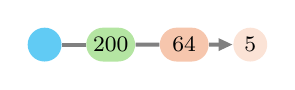
\begin{tikzpicture}[node distance=\nodedistance]
    % nodes
    \tikzinputnode{input}   at (0, 0)           (input)   {};
    \tikzlayernode{lstm}    [right = of input]  (1)       {200};
    \tikzlayernode{fc-relu} [right = of 1]      (2)       {64};
    \tikzinputnode{fc}      [right = of 2]      (output)  {5};

    % arrows
    \draw[connector]  (input) -- (1);
    \draw[connector]  (1)     -- (2);
    \draw[arrow]      (2)     -- (output);
  \end{tikzpicture}
  \caption{An example of NN architecture with the symbols defined in table \ref{tab:notations}}
  \label{fig:example-architecture}
\end{figure}
For example, figure \ref{fig:example-architecture} illustrates an architecture with
\begin{enumerate}
  \item an input (Google Stock Price data in this case),
  \item an LSTM layer with 400 units,
  \item a fully connected layer with 64 units and ReLU activation, and
  \item a fully connected layer with 5 units as an output.
\end{enumerate}

%-------------------------------------------------------------------------
\subsection{Model Training}

All models were developed in Python TensorFlow with model workloads executed on a GPU and a random seed of 112.
The same set of hyperparameters and architectures in table \ref{tab:hyperparameters} were used to train on each
target.
\begin{table}[!ht]
  \centering
  \caption{Hyperparameters used to train and tune the models}
  \label{tab:hyperparameters}
  \begin{tabularx}{\columnwidth}{Lp{89pt}}
    \rowcolor{lightgray}
    \bf Parameter           & \bf Value(s) \\
    \bhline
    Number of iterations    & 10,000,000, stopping after no improvement in 20 iterations on the validation set \\
    \evenrow
    Learning rate           & [0.1, 0.01] \\
    Number of observed days & [15, 30, 45, 60, 90] \\
    \evenrow
    Batch size              & Equal to the number of records in a train set \\
    Architecture            & 7 architectures (see Appendix \ref{appendix:architectures})
  \end{tabularx}
\end{table}
The best configuration for each target was then chosen based on the MSE on the validation set.

%-------------------------------------------------------------------------
\section{Code}

The implementation can be found \href{https://github.com/wvjgsuhp/deep-learning-fundamentals-ass-3}{here}.

%-------------------------------------------------------------------------
\section{Results}

%-------------------------------------------------------------------------
\subsection{EDA}

\begin{figure}[!ht]
  \centering
  \includegraphics[width=\columnwidth]{../assets/simple_plot.pdf}
  \caption{Line plot of Google Stock Price dataset}
  \label{fig:simple-plot}
\end{figure}
Figure \ref{fig:simple-plot} shows that for a period, close prices are around 2 times of other prices. This
could be caused by incorrect data collection. To address this, the close prices were divided by 2 as illustrated
inf Figure \ref{fig:adjust-plot}.
\begin{figure}[!ht]
  \centering
  \includegraphics[width=\columnwidth]{../assets/adjust_plot.pdf}
  \caption{Line plot of Google Stock Price dataset}
  \label{fig:adjust-plot}
\end{figure}
There was no anomaly in volume data that can be seen in Appendix \ref{appendix:volume}.

%table for best performance
\input{./best-performance.tex}

%-------------------------------------------------------------------------
\subsection{Overall MSE}

Figure \ref{fig:overall-performance} shows that the MSEs of all target prices share a similar wide spread,
around 300 - 70,000, across different configurations. This means that getting acceptable MSEs depend heavily on
picking the right architecture with right hyperparameters.
\begin{figure}[!ht]
  \centering
  \includegraphics[width=\columnwidth]{../assets/violin_plot.pdf}
  \caption{MSEs of models with different target prices on the validation set}
  \label{fig:overall-performance}
\end{figure}

%-------------------------------------------------------------------------
\subsection{Best Performance}

From table \ref{tab:price-performance}, the configuration with the lowest MSE for predicting next 5 close, low
,and open prices requires only 15 prior days to be observed while that for predicting high prices takes 45 prior
days. The best architectures for predicting these prices are all different with the architecture used for the
close prices being the simplest one with only one hidden LSTM layer. On the other hand, the architectures for
other prices consist of at least two LSTM layers. Additionally, the observed performance on test set is much
worse than that of the validation set.

%-------------------------------------------------------------------------
\subsection{Example Prediction}

\begin{figure}[!ht]
  \centering
  \includegraphics[width=\columnwidth]{../assets/example_plot.pdf}
  \caption{Predictions of high prices}
  \label{fig:example-plot}
\end{figure}
Figure \ref{fig:example-plot} shows that predictions are slightly more accurate on the first 3 days of the
predicted days for high prices. Notably, prediction accuracy is falling off after around 100 time periods in the
validation set. This signals that we could experiment with shorter train and validation sets.

%-------------------------------------------------------------------------
\section{Conclusion}

The results in this work show that using LSTM layers to predict Google Stock Price data requires more fine
tuning before it can go to real-world application. To extend this work, we could
\begin{enumerate}
  \item use different metrics and loss functions,
  \item explore shorter periods of train and validation sets,
  \item predict different numbers of days into the future,
  \item use several different stock price datasets, and
  \item experiment with different hyperparameters and architectures.
\end{enumerate}

%-------------------------------------------------------------------------
\clearpage
\begin{appendices}
\section{}
\label{appendix:architectures}

\subsection{Neural Network Architectures}

\def\modelbaseline{-0.15cm}
\begin{enumerate}[itemsep=0.5cm]
  \item \architecturea{\modelbaseline}
  \item \architectureb{\modelbaseline}
  \item \architecturec{\modelbaseline}
  \item \architectured{\modelbaseline}
  \item \architecturee{\modelbaseline}
  \item \architecturef{\modelbaseline}
  \item \architectureg{\modelbaseline}
\end{enumerate}

\section{}
\label{appendix:volume}

\subsection{Plots}

\begin{figure}[!ht]
  \centering
  \includegraphics[width=\columnwidth]{../assets/volume_plot.pdf}
  \caption{Volume of Google Stock Price dataset}
  \label{fig:volume-plot}
\end{figure}

\end{appendices}

%------------------------------------------------------------------------
\bibliography{references.bib}

\end{document}
